

\title{Schlüsselexperimente in der Teilchenphysik}
\author{
        Jean-Marco Alameddine \\
}
\date{\today}

\documentclass[12pt]{article}

% deutsche Spracheinstellungen
\usepackage{polyglossia}
\setmainlanguage{german}

\usepackage{suffix}

\usepackage{geometry}
\geometry{a4paper,left=25mm,right=25mm, top=3cm, bottom=3cm}

% unverzichtbare Mathe-Befehle
\usepackage{amsmath}
% viele Mathe-Symbole
\usepackage{amssymb}
% Erweiterungen für amsmath
\usepackage{mathtools}

% Fonteinstellungen
\usepackage{fontspec}
% Latin Modern Fonts werden automatisch geladen

\usepackage[
  math-style=ISO,    % ┐
  bold-style=ISO,    % │
  sans-style=italic, % │ ISO-Standard folgen
  nabla=upright,     % │
  partial=upright,   % ┘
  warnings-off={           % ┐
    mathtools-colon,       % │ unnötige Warnungen ausschalten
    mathtools-overbracket, % │
  },                       % ┘
]{unicode-math}

% traditionelle Fonts für Mathematik
\setmathfont{Latin Modern Math}
\setmathfont{XITS Math}[range={scr, bfscr}]
\setmathfont{XITS Math}[range={cal, bfcal}, StylisticSet=1]

% Zahlen und Einheiten
\usepackage[
  locale=DE,                 % deutsche Einstellungen
  separate-uncertainty=true, % immer Fehler mit \pm
  per-mode=reciprocal,       % ^-1 für inverse Einheiten
  % alternativ:
  % per-mode=reciprocal, % m s^{-1}
  % decimal-marker=., % . statt , f�r Dezimalzahlen
]{siunitx}

% chemische Formeln
\usepackage[
  version=4,
  math-greek=default, % ┐ mit unicode-math zusammenarbeiten
  text-greek=default, % ┘
]{mhchem}

% Grafiken können eingebunden werden
\usepackage{graphicx}
% größere Variation von Dateinamen möglich (Probleme mit Leerzeichen behoben)
\usepackage{grffile}

\usepackage{float}

\newcommand\chapterauthor[1]{\authortoc{#1}\printchapterauthor{#1}}
\WithSuffix\newcommand\chapterauthor*[1]{\printchapterauthor{#1}}

\makeatletter
\newcommand{\printchapterauthor}[1]{%
  {\parindent0pt\vspace*{-25pt}%
  \linespread{1.5}\large\scshape#1%
  \par\nobreak\vspace*{35pt}}
  \@afterheading%
}
\newcommand{\authortoc}[1]{%
  \addtocontents{toc}{\vskip-5pt}%
  \addtocontents{toc}{%
    \protect\contentsline{chapter}%
    {\hskip1.3em\mdseries\scshape\protect\scriptsize#1}{}{}}
  \addtocontents{toc}{\vskip5pt}%
}
\makeatother

\usepackage{xfrac}

\begin{document}

\maketitle
\newpage

%\begin{abstract}
%This is the paper's abstract \ldots
%\end{abstract}

\tableofcontents
\newpage

\section{Cherenkov-Detektoren}

\chapterauthor{Rune Dominik, 26.10.2018}

\subsection{Geschichte}
Tatsächlich hat bereits Marie Curie blaues Licht gesehen, was heute als Cherenkovlicht erklärt werden kann.

\subsection{Theorie}
Der Cherenkoveffekt tritt auf, wenn geladene Teilchen mit Überlichtgeschwindigkeit durch ein Medium propagieren. Es wird hierdurch ein Cherekovlichtkegel abgegeben, siehe Abbildung \ref{fig:aufbau}.

\begin{figure}[H]
  \centering
  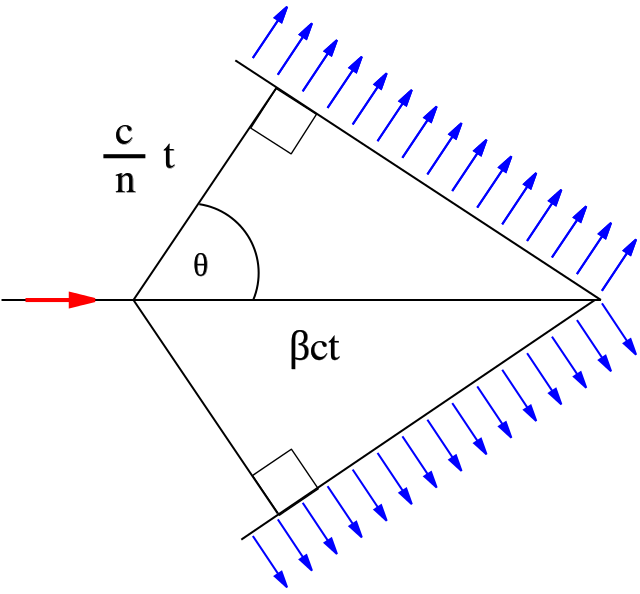
\includegraphics[height=6.0cm]{content/Cherenkov.png}
  \caption{Theoretische Erklärung des Cherenkoveffektes.}
  \label{fig:aufbau}
\end{figure}

\subsection{Aufbau}
Es gibt verschiedene Bauweisen für solche Teleskope. Insbesondere die HESE ist eine sehr moderne Bauweise.

Test~\cite{Gil:02}



\newpage


\section{Wu-Experiment}

\chapterauthor{Inga Höfmann, 02.11.2018}

\subsection{Historische Entwicklung}
Das Wu-Experiment beschäftigt sich mit der Parität, welche als Operator eine Inversion in allen Raumkoordinaten beschreibt. Es gilt
\begin{align*}
	\hat{P} \vec{r} &= -\vec{r}, &
	\hat{P} \vec{L} &= \vec{L}.
\end{align*}
Die Parität wurde erstmals im Jahre 1927 als Quantenzahl und somit intrinsische Eigenschaft eines Teilchen eingeführt und galt zunächst für alle Wechselwirkungen als erhalten.
Zweifel an der Parität als Erhaltungsgröße kamen im Jahr 1954 mit dem sogenanten $\tau$-$\theta$-Puzzle auf:
Die damals als $\tau$- und $\theta$-Meson bekannten Teilchen besaßen identische Massen, Ladungen und Lebensdauern.
Unteschiede ergaben sich lediglich in den Zerfallsprodukten:
Während das $\tau^+$-Meson in den Endzustand $\pi^+ \pi^+ \pi^-$ (Parität $-1$) zerfiel, war der Endzustand des $\theta^+$-Mesons $\pi^+ \pi^0$ (Parität $+1$).
Als Erklärung dieses Puzzles existierte die Möglichkeit, dass es sich bei beiden Mesonen um das gleiche Teilchen handelt und die Parität in diesem Fall verletzt ist.
Diese Vermutung wurde, zusammen mit Vorschlägen für einen experimentellen Aufbau, im Jahre 1957 von Tsung-Dao Lee und Chen Ning Yang in einem Paper veröffentlicht, wofür sie 1957 den Nobelpreis erhielten.
Das dazugehörige Experiment wurde von der Physikerin Chien-Shiung Wu im Jahre 1956 innerhalb von neun Monaten realisiert.

\subsection{Idee des Wu-Experimentes}
Die Idee des Wu-Experimentes ist es, eine Paritätsverletzung in der schwachen Wechselwirkungs nachzuweisen.
Um einen Interferenzterm mit paritätserhaltenden und paritätsverletzenden Anteilen untersuchen zu können muss eine pseudoskalare Messgröße genutzt werden.
Hierzu bietet es sich an, die Winkelverteilung $I\left(\theta \right)$ von $e^-$ in einem $\beta$-Zerfall zu betrachten. 
Es ergibt sich ein Parameter $\alpha$, welcher die Asymmetrie in der Winkelverteilung beschreibt, wobei $\alpha = 0$ für Paritätserhaltung bzw. $\alpha \neq 0$ für Paritätsverletzung gilt.

Das Wu-Experiment ist so konzipiert, dass es rein qualitative Aussagen über den Parameter $\alpha$ treffen kann.
Als Probe wird $\ce{^{60}_{27}Co}$ verwendet, welches dominant unter Aussendung eines $e^-$ und eines $\bar{\nu_e}$ (d.h. unter der schwachen Wechselwirkung) in $\ce{^{60}_{28}Ni^{*}}$ zerfällt. Dieses sendet widerum zwei energetisch charakteristische Photonen aus um in einen nicht angeregten Zustand zu gelangen.
Zu beachten ist, dass $\ce{^{60}_{27}Co}$ einen Spin von $5$ und $\ce{^{60}_{28}Ni^{*}}$ einen Spin von $4$ besitzt.
Somit müssen die Ausrichtungen der Spin-$z$-Komponente des $e^-$, des $\bar{\nu_e}$ (beide mit Spin $\sfrac{1}{2}$) und des $\ce{^{60}_{28}Ni^{*}}$ alle in die gleiche Richtung zeigen.
Werden die Spins der Kobalt-Atome nun in eine Vorzugsrichtung ausgerichtet, kann die Anzahl der Elektronen in Spinrichtung gemessen werden.
Wird die Vorzugsrichtung der Spins umgekehrt, was einer Paritätstransformation entspricht, so wird die Anzahl der Elektronen gegen die Spinrichtung gemessen.
Somit wird die Messung einer möglichen Paritätsverletzung ermöglicht.

\subsection{Experimentelle Herausforderungen}
Insbesondere die Ausrichtung der Spins der Kobalt-Atome stellt eine große experimentelle Herausforderung dar.
Hierfür werden sowohl sehr geringe Temperaturen ($\approx \SI{1}{\kelvin}$) als auch hohe Magnetfelder ($\approx \SI{10}{\tesla}$) benötigt.
Die Lösung stellte die sogenannte Rose-Gorter-Methode dar.
Hierbei wird ein Kristall, $\ce{CeMg}$-Nitrat, verwendet, wobei das Salz einen anistotropen $g$-Faktor besitzt.
Die starke Abkühlung geschieht durch das Anlegen eines B-Feldes entlang des maximalen $g$-Faktors.
Zunächst werden dabei die, aufgrund der Hyperfeinstrukturaufspaltung entstehenden, niedrigeren Energieniveaus besetzt.
Anschließend wird das System thermisch isoliert und das Magnetfeld heruntergefahren.
Durch diese sogenannte adiabatische Entmagnetisierung können hinreichend geringe Temperaturen erreicht werden.
Das Anlegen eines Magnetfeldes in Richtung des minimalen $g$-Faktors ermöglicht dann die Polarisation der Hüllenelektronen des Kobalts.
Dies führt zu einer starken Zunahme des $B$-Feldes in der Nähe des Kerns und somit zu einer Polarisation der Spins der Kerne.
Werte der Polarisation von bis zu $\SI{60}{\percent}$ konnten hiermit erreicht werden.
Die experimentelle Realisierung ist in Abbildung \ref{fig:wu} dargestellt.

\begin{figure}
  \centering
  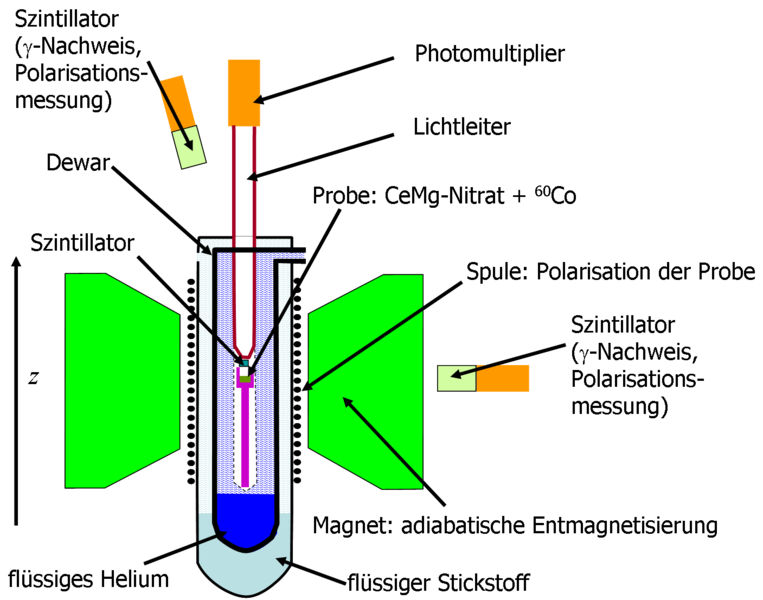
\includegraphics[height=7.0cm]{ressources/wu.png}
  \caption{Schematischer Aufbau des Wu-Experimentes \cite{wu}.}
  \label{fig:wu}
\end{figure}

Die Polarisation des Kernspins geschieht über die $\gamma$-Szintillatoren, da die Photonen vorzugsweise in Spin-Richtung emmitiert werden.
Der Nachweis der Elektronen geschieht direkt über den Szintillatorkristall über Photomultiplier.
Um die Parität untersuchen zu können wird das gesamte Experiment mit zwei verschiedenen Ausrichtungen des Magnetfeldes und somit mit zwei verschiedenen Vorzugsrichtungen der Spins durchgeführt.

\subsection{Experimentelle Ergebnisse und Konsequenzen}
Experimentell konnte nachgewiesen werden, dass die Kernspins hinreichend polarisiert werden konnten.
Zudem wurde gezeigt, dass die Elektronen vorzugsweise gegen die Richtung des Kernspins des Kobalts emmitiert werden.
Dies entspricht einer Verletzung der Parität und bestätigte somit die These von Tsung-Dao Lee und Chen Ning Yang.
Spätere Experimente wiesen quantitativ nach, dass die Parität tatsächlich maximal verletzt ist.
Zudem folgte die theoretische Erkenntnis, dass die schwache Wechselwirkung eine V-A-Struktur besitzt:
Sie koppelt nur an linkshändige Teilchen und rechtshändige Antiteilchen, was die maximale Paritätsverletzung erklärt.

\subsection{Diskussion zum Vortrag}
Als Frage wurde gestellt, ob die Suche nach Paritätsverletzung in anderen Wechselwirkungen ebenfalls durchgeführt wurde.
Hierbei ergab sich die Antwort, dass bis heute nach paritätsverletzenden Anteilen außerhalb der schwachen Wechselwirkung gesucht wird.

Da Kobalt zwei unteschiedliche $\beta^-$-Zerfallsmoden in Nickel besitzt, kam die Frage auf wie diese Unterschiede experimentell berücksichtigt wurden.
Dies war möglich und wurde realisiert, da die Szinzillatoren auf die festen Energien der Photonen ausgerichtet werden können.

Zuletzt wurde über technische Details der Kühlung diskutiert.
Hierbei wurde das Pumpen erwähnt, welches genutzt wurde, um eine Kühlung auf bis zu $\SI{1}{\kelvin}$ zu ermöglichen.

\newpage


\section{Die Entdeckung des Gluons}

\chapterauthor{Dominik Hellmann, 09.11.2018}

\subsection{Theoretische Grundlagen der Quantenchromodynamik}
Die Quantenchromodynamik (QCD) ist die Quantenfeldtheorie der starken Wechselwirkung, d.h. der Kraft, die für das Zusammenhalten der Quarks in Hadronen verantwortlich ist.
Grundlage für die QCD ist die Yang-Mills-Theorie, welche eine im Jahre 1954 entwickelte Eichtheorie ist.
Dabei folgt die QCD aus der $SU(3)_\text{c}$-Symmetriegruppe, wobei hieraus die drei Farbladungen rot, grün, blau und die dazugehörigen Antifarben resultieren.
Die Farben sind dabei analog zu den elektrischen Ladungen der QED zu verstehen.

Analog zu den Photonen der QED existieren auch Eichbosonen der QCD, welche Gluonen heißen.
Aus der Gruppentheorie folgt, dass 8 Gluonen existieren, welche den Generatoren der $SU(3)_\text{c}$ entsprechen.
Gluonen sind masselose Vektorteilchen, welche jedoch im Kontrast zur QED ebenfalls Farbladung besitzen und dementsprechend an sich selbst koppeln können.
Hieraus folgt die asymptotische Freiheit als charakteristische Eigenschaft der QCD:
Durch Vakuumpolarisationen, dem sogenannten Anti-Screening, wird die Kopplungskonstante der QCD $\alpha_{s}$ klein für große Impulsübertäge. 
Hieraus folgt, dass die einzelnen Quarks bei großen Impulsübertägen, bzw. kleinen Abständen, als asymptotisch frei verstanden werden können.
Andereresits folgt als Charakteristikum das Confinement: Bei großen Abständen steigt das Potential der QCD linear an, d.h. die Kraft für das weitere Vergrößern des Abstandes wächst linear.
Wird der Abstand weiter vergrößert, so werden neue Teilchen in sogenannten Jets produziert, bis der Endzustand wieder farbneutral ist.
Dementsprechend können farbgeladene Teilchen nur in einem farbneutralen, gebundenen Zustand beobachtet werden.
Die entstehenden Jets können in einem Detektor als Ansammlung von Teilchen beobachtet werden, wobei die Messung der Impulse aller beobachteten Teilchen Rückschlüsse auf die Impulse der ursprünglichen Quarks zulässt.

\subsection{Historische Entwicklung}

Im Jahr 1964 wurden von Murray Gell-Mann erstmals Quarks als Bestandteile der Hadronen postuliert.
Hierbei stellen sich die Fragen, welche Kräfte diese Elementarteilchen zusammenhalten und welche Austauschteilchen diese Kraft vermitteln.
Weitere Hinweise auf eine mit der QCD verbundenen Quantenzahl stellten die $\Delta$-Baryonen sowie der $R$-Plot dar.
So ist die Wellenfunktion des $\Delta^{++}$-Baryons unter Vertauschung von zwei Quarks symmetrisch, falls nur die bisher bekannten Raum-, Flavor- und Spinanteile der Wellenfunktion berücksichtigt werden.
Dies steht jedoch im Widerspruch mit dem Pauliprinzip für Fermionen.
Die Einführung einer Farbe als Quantenzahl stellt den nötigen antisymmetrischen Anteil der Wellenfunktion bereit und löst somit dieses Problem.

Bei der Betrachtung des $R$-Plots wird die Häufigkeit der Produktion von Hadronen in $e^+ e^-$ Reaktionen in Abhängigkeit von der Schwerpunktsenergie betrachtet.
Hierbei ist das Verhältnis $R$ sensitiv auf das Vorhandensein von Farbladungen und sagt experimentell drei Farbladungen vorraus.

\subsection{Jetphysik am DESY}
Das DESY (Deutsche Elektron Synchrotron) ist ein Forschungszentrum für Teilchenphysik, welches 1959 in Hamburg gegründet wurde.
Der dort gebaute $e^+ e^-$ Collider PETRA (Positron-Electron-Tandeom-Ring Accelerator) wurde im Oktober 1978 in Betrieb genommen.
Mit einem Umfang von $U=\SI{2.3}{\kilo\metre}$ konnten im späteren Betrieb Schwerpunktsenergien von bis zu $\SI{47}{\giga\electronvolt}$ erreicht werden.
Eines der an diesem Collider arbeitenden Experimente war TASSO (Two Arm Spectrometer Solenoid).
Mithilfe des mit einem Magnetfeld durchsetzten Zentraldetektors war eine genaue Impulsmessung möglich, zur Geschwindigkeitsmessung wurde ein Flugzeitzählersystem verwendet.
In den beiden Armen des Detektors konnte durch drei Lagen von Schwellen-Cherenkovzählern, Schauerzählern sowie den Flugzeitzählerystemen eine sehr gute Teilchenidentifikation ermöglicht werden.

Die Jet-Rekonstruktion zu dieser Zeit konzentrierte sich insbesondere auf die Beobachtung von 2-Jet-Ereignissen, wie sie 1975 durch Feynman erstmals vorhergesagt und 1978 am DESY entdeckt wurden.
Im Rahmen des Cone-Algorithmus wird dabei eine Hauptjetachse gesucht und die Impulse entlang dieser Achse maximiert beziehungsweise die Impulse transversal zu der Hauptachse minimiert.
Um die Existenz von Gluonen in der QCD zu beweisen kann das Auftreten von 3-Jet-Strukturen verwendet werden.
Dies entspricht der Abstrahlung eines Gluons, wie in Abbildung \ref{fig:gluon} dargestellt ist.
\begin{figure}
  \centering
  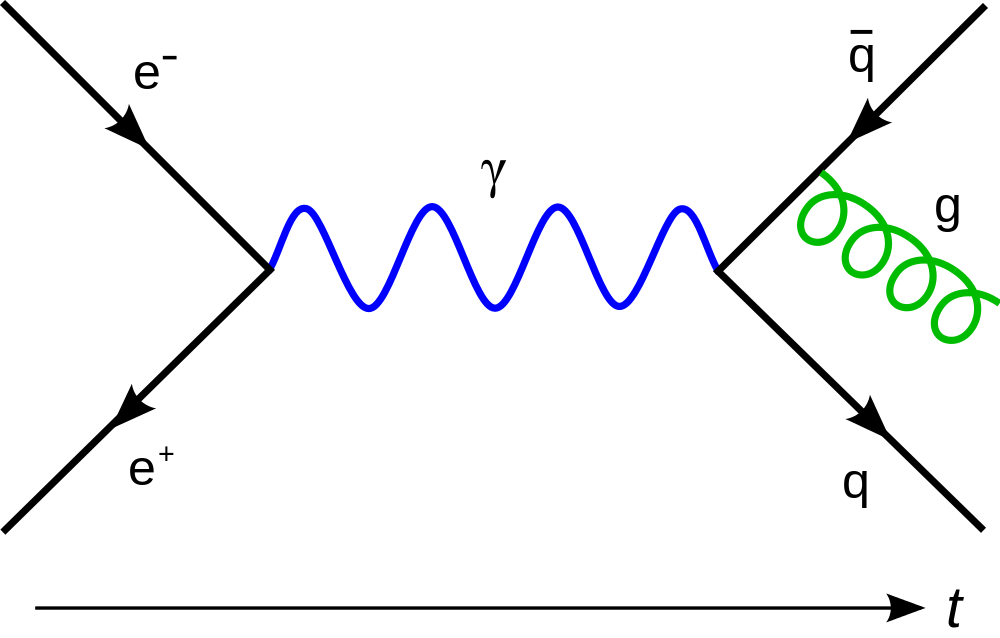
\includegraphics[height=4.0cm]{ressources/gluon.png}
  \caption{Abstrahlung eines Gluons in einer $e^+ e^-$-Kollision \cite{gluon}.}
  \label{fig:gluon}
\end{figure}
Bei einem ausreichend großen Tansversalimpuls des Gluons entsteht ein dritter Jet, der im Detektor nachgewiesen werden kann.

\subsection{Analyse der Jets der TASSO-Kollaboration}
Die Analyse der Jets wurde von der TASSO-Kollaboration bei verschiedenen Schwerpunktsenergien durchgeführt. 
Dabei teilt sich die Analyse jeweils in verschidene Schritte auf.
Zunächst wird die Hauptjetachse durch das Maxmimeren des Impulses in die Jetachsenrichtung bestimmt.
Die Verteilung der Impulse transversal zur Hauptsachse wird nun untersucht, wobei hier einer energieabhängige Verteilung der Transveralimpulse beobachtet wurde, die mit der Schwerpunktsenergie zugenommen hat. 
Dies widerspricht den bisherigen naiven Partonmodellen und ließe sich beispielsweise über die Abstrahlung von Gluonen erklären.

Im nächsten Schritt werden die Breiten der einzelnen Jets untersucht.
Bei zwei rekonstruierten Jets wäre zu erwarten, dass jeweils nur ein Jet aufgrund von Gluonabstrahlung verbreitert ist und somit eine Asymmetrie zu beobachten ist.
Die Ergebnisse zeigen, dass die Asymmetrie für größere Schwerpunktsenergien ansteigt und somit für verschiedene Energien unterschiedliche Parameter der Quark-Parton-Modelle verwendet werden müssen.
Auch dieses Verhalten ist mit der Abstrahlung von Gluonen als Erklärung kompatibel.

Der letzte Schritt besteht darin, die Struktur der 3-Jet-Ereignisse eindeutig von den kolinearen 2-Jet-Ereignissen zu trennen.
Dabei müssen die drei beobachteten Jets aufgrund der Impulserhaltung in einer Ebene liegen, jedoch eine Abweichung von der kolinearen Struktur innerhalb dieser Ebene aufweisen.
Dazu wird aus den beobachteten Impulsen der Hadron-Impulstensor ermittelt.
Aus den Eigenvektoren dieses Tensors lassen sich die Größen $\left<p_T^2\right>_\text{in}$ und $\left<p_T^2\right>_\text{out}$ ermitteln welche jeweils angeben, wie stark die gemessenen Impulse aus der Ereignisebene herausragen bzw. wie stark die Impulse von der Hauptjetachse in der Ereigbnisebene abweichen.
Beobachtet wird, dass $\left<p_T^2\right>_\text{out}$ lediglich einen geringen Anstieg mit der Schwerpunksenergie aufzeigt, während sich $\left<p_T^2\right>_\text{in}$ bei höheren Energien nicht mehr korrekt mit dem naiven Quark-Parton Modell beschreiben lässt.
Dies deutet auf ein drittes farbgeladenes Teilchen im Endzustand, welches bei höheren Energien einen Jet erzeugt, wobei die Häufigkeit dieser Ereignisse nicht mehr mit statistischen Fluktuationen kompatibel ist.

Der somit bestätigten Existenz des Gluons folgte die Bestimmung seines Spins, welches laut Theorie den Wert $1$ besitzen sollte.
Als hiermit korrelierte Größe wurde 1980 der sogenannte Ellis-Karliner Winkel von der TASSO-Kollaboration gemessen und mit Simulationen für verschiedene Spins des Gluons verglichen.
Hierbei wurde eine gute Übereinstimmung mit der Annahme eines Vektorteilchens, d.h. Spin 1 des Gluons, ermittelt.
Es folgten weitere Spinmessungen der SLD Kollboration, die dieses Ergebnis bestätigten.

\subsection{Heutige Jetphysik und QCD-Forschung}

In der heutigen Jetphysik können in einem Ereignis aufgrund der höheren Schwerpunktsenergien der Beschleuniger deutlich mehr als zwei Jets beobachtet werden.
Hierzu werden effiziente und schnelle Rekonstruktionsalgorithmen benötigt, welche die Eigenschaften der Infrarot-Stabilität sowie der kollinearen Stabilität erfüllen müsen.
Dafür werden, im Vergleich zu den vorher verwendeten Cone-Algortihmen, heutzutage häufig sequentielle Cluster Algorithmen (beispielsweise $k_t$, anti-$k_t$ und Camebridge/Aachsen) verwendet.

Aktuelle Forschungsfragen der QCD sind beispielsweise die Existenz von Glueballs oder der Beitrag der Gluonen und verschiedenen Quarks zum Protonspin.

\subsection{Diskussion}
Im Anschluss des Vortrages wurde gefragt, inwiefern sich die unterschiedlichen Spinmessungen des Gluons der verschiedenen Kollaborationen unterschieden haben.
Beim Folgeexperiment der SLD Kollaboration wurde durch höhere Schwerpunktsenergien und einen besseren Detektor eine höhere Auflösung und somit eine genauere Messung ermöglicht.

Zudem wurde gefragt, ob andere Kandidaten neben der QCD zur Erklärung der starken Wechselwirkung existierten.
Zwar wäre es möglich gewesen, einige Ergebnisse der Experimente zur Suche nach Gluonen durch einen weiteren Quarkflavor zu erklären - dies wurde jedoch bereits früh durch andere Experimente bei den geringen, hier genutzen Schwerpunktsenergien ausgeschlossen.
Eine generelle alternative theoretische Erklärung der starken Wechselwirkung exisiterte jedoch nicht.
\newpage

\bibliographystyle{abbrv}
\bibliography{summary}

\end{document}

